\documentclass[12pt,aspectratio=169]{beamer}
\usepackage{fancyvrb}
\RecustomVerbatimCommand{\VerbatimInput}{VerbatimInput}{frame=single,
numbersep=1mm, numbers=left, formatcom=\color{orange}}
%\usepackage{kpfonts}
%\usepackage[bitstream-charter]{mathdesign}
\usepackage[utf8]{inputenc}
\usepackage{pgf}
\usepackage{verbatim}
%\usepackage{fontspec}
\usepackage[ruled,vlined,linesnumbered]{algorithm2e}
\IncMargin{1em}
\usetheme{Madrid}
\setbeamerfont{frametitle}{series=\bfseries}
\usecolortheme[dark]{solarized}
\setbeamertemplate{blocks}[rounded][shadow=false]
\setbeamertemplate{navigation symbols}{}

\author{Gianluca Della Vedova}
\title[Advanced Algorithms]{Advanced Techniques for Combinatorial Algorithms:
Parallel Algorithms}
\institute[]{Univ. Milano -- Bicocca\\
  \texttt{https://gianluca.dellavedova.org}}


\DeclareMathOperator{\poly}{\text{poly}}
\DeclareMathOperator{\polylog}{\text{polylog}}


% If you wish to uncover everything in a step-wise fashion, uncomment
% the following command:
\beamerdefaultoverlayspecification{<+->}


\begin{document}

\begin{frame}
  \titlepage
\end{frame}





\begin{frame}\frametitle{RAM model}
  \begin{itemize}
  \item
    Random Access Memory
  \item
    One processor
  \item
    sequential algorithms
  \item
    Flat memory
  \item
    Infinite memory
  \end{itemize}
\end{frame}

\begin{frame}\frametitle{PRAM model}
  \begin{itemize}
  \item
    \alert{Parallel} RAM
  \item
    $p$ RAMs
  \item
    Shared memory
  \item
    Synchronized (running on the same clock)
  \end{itemize}
\end{frame}

\begin{frame}\frametitle{PRAM model}
  \begin{itemize}
  \item
Parallel computation is \alert{rapidly} becoming a \alert{dominant} theme in all areas of
computer science and its applications.
It is likely that, \alert{within a decade}, virtually all developments in computer
architecture, systems programming, computer applications and the design of
algorithms will be taking place within the context of parallel computation.
\item
\small  Karp, R M. and Ramachandran, V. Chapter 17. Parallel Algorithms for
  Shared-Memory Machines. Handbook of Theoretical Computer Science: Algorithms and complexity, Volume 1.
 \alert{1990}.
\end{itemize}
\end{frame}


\begin{frame}\frametitle{PRAM model}
  \begin{itemize}[<.->]
    \item
Selim Akl, Parallel Computation: Models and Methods, Prentice Hall, 1997.    
    \item
Selim Akl, Design \& Analysis of Parallel Algorithms, Prentice Hall, 1989.
    \item
Cormen, Leiserson, and Rivest, Introduction to Algorithms, 1st edition,
1990, McGraw Hill and MIT Press, Chapter 30 on parallel algorithms.
    \item
Joseph JaJa, An Introduction to Parallel Algorithms, Addison Wesley, 1992.
\end{itemize}
\end{frame}

\begin{frame}\frametitle{PRAM model}
  \begin{itemize}
  \item
    It's a \alert{MODEL}!
  \item
    MIMD (Multiple Instruction Multiple Data)
  \item
    Processor ID
  \item
      No communication cost
  \item
      Shared memory, same access time
  \end{itemize}
\end{frame}

\begin{frame}\frametitle{PRAM model}
% This LaTeX table template is generated by emacs 24.1.50.1
\begin{center}
  \begin{tabular}{|l|l|l|}
\hline
 & Read & Write \\
\hline
Exclusive & ER & EW \\
\hline
Concurrent & CR & CW \\
\hline
\end{tabular}

\begin{itemize}
\item
  Different accesses
  \item
    CRCW is better than EREW.
  \item
    But how much?
\item
    There are different CRCW models:
    \begin{itemize}
  \item
    Common CRCW: concurrent writes if same value from all processors
  \item
    Priority CRCW: highest priority processor wins
    \end{itemize}
\end{itemize}
\end{center}
\end{frame}


\begin{frame}\frametitle{Efficient Algorithm}
\begin{itemize}
\item
  $t(n)$ = polylogarithmic time
\item
  $p(n)$ = polynomial number of processors
\item
  $\mathbf{NC}$
\item
  $\mathbf{NC}\subseteq \mathbf{P}$
\item
  Hardness = $\mathbf{P}$-complete problems
\end{itemize}
\end{frame}



\begin{frame}\frametitle{Simulations}
\begin{itemize}
\item
  EREW PRAM can simulate CRCW PRAM
\item
  Time multiplied by $O(\log p(n))$
\end{itemize}
\end{frame}


\begin{frame}\frametitle{Optimal Algorithm}
\begin{itemize}
\item
  \alert{work} $w(n) \le t(n) p(n)$
\item
  $t(n)$ = polylogarithmic time
\item
  $w(n) = O(T(n))$, where $T(n)$ = time complexity of \alert{best known}
  sequential algorithm
\end{itemize}
\end{frame}



\section{Algorithms}


\begin{frame}\frametitle{}
  \begin{center}
    \Huge
    Algorithms
  \end{center}
\end{frame}
\begin{frame}\frametitle{Sum of elements of an array}
\begin{algorithm}[H]
\SetKwData{Array}{$x[1], \ldots , x[n]$}
\eIf{$n=1$}{
  \Return $x[1]$
}{
  \Return Sum($\{x[2i-1] + x[2i] : 1\le i\le n/2\}$)
}
\caption{Sum}
\end{algorithm}

\begin{algorithm}[H]
\SetKwData{Array}{$x[1], \ldots , x[n]$}
\For{$i\gets 1$ \KwTo $n$ in parallel}{
  $B[i] \gets x[i]$
}
\For{$k\gets 1$ \KwTo $(\log_{2} n) - 1$}{
  \For{$i\gets 1$ \KwTo $2^{k - 1}$ in parallel}{
    $B[i] \gets B[i] + B[i+1]$
    }
  }
\Return Sum($\{x[2i-1] + x[2i] : 1\le i\le n/2\}$)
\caption{Iterative Sum}
\end{algorithm}
\end{frame}


\begin{frame}\frametitle{Prefix sum problem (PRAM)}
  \begin{itemize}
  \item
    Input
  \item
    Sequence $\langle x_{1}, \ldots , x_{n} \rangle$ of elements
  \item
    Associative operation $+$
  \item
    Output
  \item
     $S=\langle S_{1}  \ldots , S_{n} \rangle$, with $S_{i} = x_{1} +
     \cdots + x_{i}$
   \item
     trivial sequential algorithm
  \end{itemize}
\end{frame}

\begin{frame}\frametitle{Prefix sum}
\begin{algorithm}[H]
\SetKwData{Array}{$x_{1}, \ldots , x_{n}$}

\For{$i\gets 1$ \KwTo $n/2$ \uncover<2>{\alert{in parallel}}}
{
  $y_{i}\gets x_{2i-1} + x_{2i}$\;
}
$S^{*} = \text{PrefixSum}([y_{1}, \ldots , y_{n/2}])$\;
\tcc{$S^{*}_{j} = x_{1} + \cdots + x_{2j}$}
\For{$i\gets 1$ \KwTo $n$ \uncover<2>{\alert{in parallel}}}
{
  \If{$i$ is even}{
    $S_{i}\gets S^{*}_{i/2}$\;
  }
  \Else{
    $S_{i}\gets S^{*}_{i/2} + x_{i}$
  }
}
\caption{PrefixSum}
\end{algorithm}
\end{frame}


\begin{frame}\frametitle{Prefix sum}
  \begin{itemize}
  \item
    EREW
  \item
    $O(\log n)$ time, $O(n)$ processors
  \item
    $w(n) = O(n)$
  \item
    $O(n/\log n)$ processors are enough
  \end{itemize}

\begin{block}{Brent's scheduling principle}
  \begin{itemize}
  \item
    $w$ work on $p$ processors in time $t$
  \item
    $p_{1}<p$ (use fewer processors)
  \item
    time $\lfloor w/p_{1}\rfloor +t$, work $w$ (more time, same work)
  \end{itemize}
\end{block}
\end{frame}

\begin{frame}\frametitle{Find Maximum}
\begin{block}{Instance}
An array $A$ of $n$ integers
\end{block}
\begin{block}{Question}
Find the largest element in $A$.    
\end{block}
\begin{block}{Goal}
Fastest algorithm
\end{block}
\end{frame}

\begin{frame}\frametitle{Find Maximum}
\begin{algorithm}[H]
\SetKwData{Array}{$x_{1}, \ldots , x_{n}$}
\For{$i\gets 1$ \KwTo $n$ in parallel}{%
  $B[i]\gets $ true\;
}
\For{$i\gets 1$ \KwTo $n$ in parallel}{%
  \For{$j\gets 1$ \KwTo $n$ in parallel}{%
    \If{$A[i] < A[j]$ or $A[i] = A[j]$ and $i < j$}{%
      $B[i]\gets $ false\;
    }
  }
}
\For{$i\gets 1$ \KwTo $n$ in parallel}{%
  \If{$B[i]$}{Return $A[i]$}
}
\caption{Find1.    
Find Maximum in an Array $A$}
\end{algorithm}
Time? Work? 
\uncover<2>{\alert{$T(n)=O(1)$, $W(n)=O(n^{2})$}}
\end{frame}

\begin{frame}\frametitle{Find Maximum}
\begin{algorithm}[H]
\SetKwData{Array}{$x_{1}, \ldots , x_{n}$}
\eIf{$n > 16$}{%
  \For{$i\gets 1$ \KwTo $\sqrt{n}$ in parallel}{%
    $B[i]\gets $Find2$(A[1 + \lfloor (i - 1)/\sqrt{n} \rfloor : \lfloor i/\sqrt{n} \rfloor])$\;
  }
  Find1($B$)\;
}{%
  Find1($A$)\;
}
\caption{Find2.    
Find Maximum in an Array $A$}
\end{algorithm}
$T(n)$ \uncover<2>{$\le T(\sqrt{n}) + c_{1} \Rightarrow T(n) = O(\log \log n)$}

$W(n)$ \uncover<2>{$\le \sqrt{n} W(\sqrt{n}) + c_{2}n \Rightarrow W(n) = O(n \log \log n)$}
\end{frame}


\begin{frame}\frametitle{Find Maximum}
\begin{algorithm}[H]
\SetKwData{Array}{$x_{1}, \ldots , x_{n}$}
\For{$i\gets 1$ \KwTo $n / \log\log n$ in parallel}{%
  $B[i]\gets \min(A[1 + \lfloor (i - 1)\log\log n \rfloor : \lfloor i/\log\log n
  \rfloor])$\;
}
Find2($B$)\;
\caption{Find3.    
Find Maximum in an Array $A$}
\end{algorithm}
$T(n) =$\uncover<2>{$ O(\log \log n)$}

$W(n) =$\uncover<2>{$ O(n)$}
\end{frame}

\begin{frame}\frametitle{Pointer Jumping}

  \begin{itemize}[<.->]
  \item
    Problem: given a single-link list L, propagate the value of the last
      element to the entire list
  \end{itemize}
\begin{algorithm}[H]
\SetKwData{List}{$L$, elements $<value, next>$}
\ForEach{$L[i]$ in parallel}{%
  \For{$k\gets 1$ \KwTo $\log_{2} n$}{%
     \If{$next(i) \neq NIL$}{%
       $next[i] \gets next[next[i]]$
    }
  }
  $value[i] \gets value$
}
\end{algorithm}
\end{frame}

\begin{frame}\frametitle{List Ranking}
  \begin{itemize}[<.->]
  \item
    Problem: given a list L, find the position of each element in L
  \end{itemize}
\begin{algorithm}[H]
\SetKwData{List}{$L$, elements $<value, next>$}
\ForEach{$L[i]$ in parallel}{%
  \eIf{$next(i) = NIL$}{%
    $rank[i] \gets 0$}{%
    $rank[i] \gets 1$
  }
  \For{$k\gets 1$ \KwTo $\log_{2} n$}{%
    $rank[i] \gets rank[i] + rank[next[i]]$\;
    $next[i] \gets next[next[i]]$
  }
}
\caption{List Ranking via pointer jumping}
\end{algorithm}
\end{frame}

\begin{frame}\frametitle{List Ranking}
\begin{block}{Proof}
  \begin{itemize}
  \item
    At iteration $k$:
  \item
    if $next[i] \neq NIL$ then $rank[i] = 2^{k}$
  \item
    if $next[i] = NIL$ then $rank[i]$ is the distance between $L[i]$ and the end of the
    list
  \item
    $next[i] = NIL$ for the last $2^{k}$ elements of $L$
  \end{itemize}
\end{block}
\end{frame}
\begin{frame}\frametitle{Binary trees}
  \begin{itemize}
  \item
    Problem: to determine depth of each node
  \item
    parent, left child, right child
  \item
    $3$ processors for each node
  \item
    $O(n)$-time sequential algorithm
  \item
    Algorithm 1: Level-wise visit, each node in parallel
  \item
    $t(n)=$height (not good)
  \end{itemize}
\end{frame}


\begin{frame}\frametitle{Euler tour}
  \begin{center}
    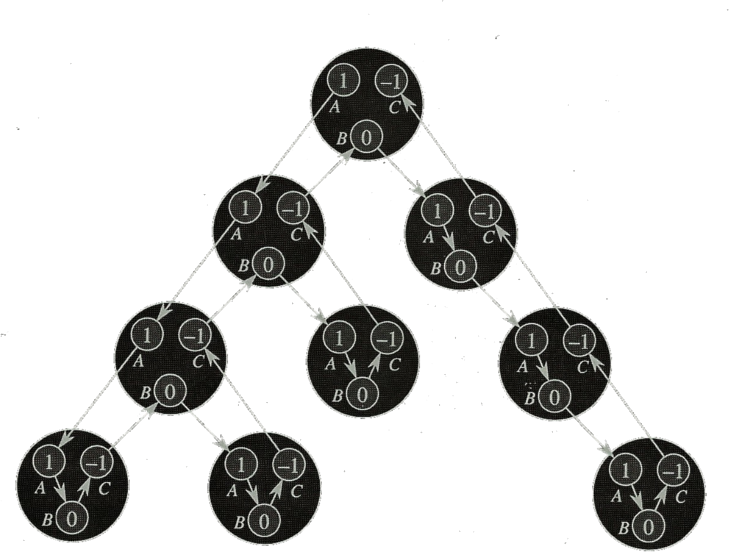
\includegraphics[width=8cm]{img/euler1}
  \end{center}

  \uncover<2>{Depth = prefix sum}
\end{frame}

\begin{frame}\frametitle{Size of all subtrees}
  \begin{center}
    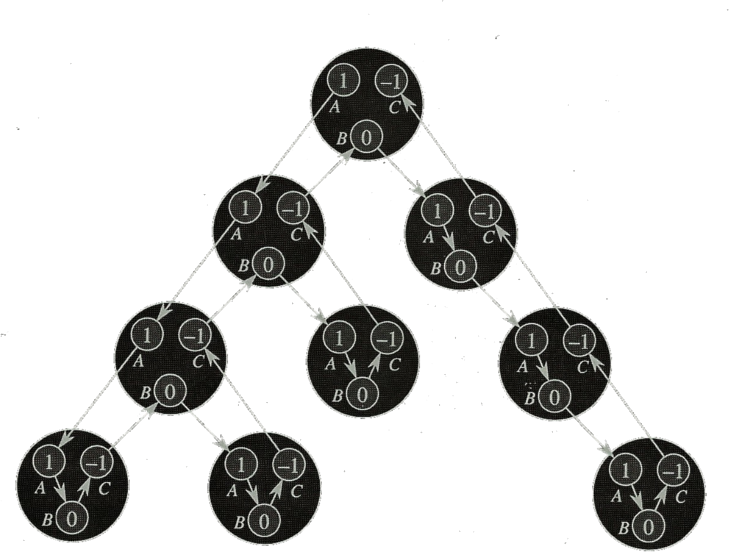
\includegraphics[width=8cm]{img/euler1}
  \end{center}

  \uncover<2>{replace $-1$ with $0$, difference between third and first prefix sums}
\end{frame}


\begin{frame}\frametitle{Matrix multiplication}
\begin{itemize}
\item
    $C = AB$, simpler case $A$, $B$ square matrices
  \item
    embarassingly parallel
  \item
    $C[i,j] = \sum_{k\le n}A[i,k]B[k,j]$
  \item
    $O(\log n)$ time, $O(n^{3}/\log n)$ processors
  \end{itemize}
\end{frame}



\begin{frame}\frametitle{Graph Algorithms}
  \begin{itemize}
  \item
    depth-first visit
  \item
    No $\mathbf{NC}$ algorithm
  \item
    breadth-first visit
  \item
    $O(n^{2.37})$ processors
  \item
    \alert{Euler tour}
  \end{itemize}
\end{frame}


\begin{frame}\frametitle{Connected components}
\begin{block}{Instance}
Undirected graph $G=(V,E)$
\end{block}
\begin{block}{Data structure}
\begin{enumerate} 
\item
$M(v,w)$ adjacency matrix
\item
$R(v) \gets v$ representative.    
All vertices in the same connected components have the same representative.    
\item
$C[v,w]$ connected components with representative $v$ and $w$ can be merged
\end{enumerate}
\end{block}
\end{frame}

\begin{frame}\frametitle{Connected components}
  \begin{algorithm}[H]
    \For(\emph{hookings}){$\log_{2} n$ times}{
    \ForEach{edge $(v,w)$ such that $R[v] \neq R[w]$}{
      \If{$R[v] < R[w]$}{%
        $C[R[v], R[w]] \gets $ true\;
      }
    }
    \ForEach{vertex $v$ such that $R[v]=v$}{
      $R[v] \gets \max w : C[R[v], R[w]]$ is true\;
    }
    \For(\emph{parallel pointer jumping}){$i\gets 1$ to $\log_{2} n$}{
      \ForEach{vertex $v$}{
        $R[v] \gets R[R[v]]$\;
      }
    }
  }
  \caption{ConnectedComponents}
  \end{algorithm}
\end{frame}


\begin{frame}\frametitle{Minimum Spanning Tree}
\begin{block}{Problem}
Given an undirected edge-weighted connected graph $G=(V,E)$, find a
minimum-weight subset
$T\subseteq E$ such that $T$ is a tree spanning $V$.    
\end{block}

\begin{block}{Lemma}
Let $G=(V,E)$ be an undirected graph, let $(V_{1}, V_{2})$ be a
bipartition of $V$, let $T$ be a minimum spanning tree of $G$, and let
$e$ be the lightest edge connecting $V_{1}$ and $V_{2}$.    
Then $e\in T$.    
\end{block}
\end{frame}


\begin{frame}\frametitle{Additional Bibliography on PRAM}

    \begin{itemize}[<.->]
    \item
A Survey of Parallel Algorithms for Shared-Memory Machines
\url{http://techreports.lib.berkeley.edu/accessPages/CSD-88-408.html}
    \item
Vishkin, Uzi (2009), Thinking in Parallel: Some Basic Data-Parallel Algorithms and
Techniques.    
\url{http://www.umiacs.umd.edu/users/vishkin/PUBLICATIONS/classnotes.pdf}    
\end{itemize}
\end{frame}


\end{document}

%%% Local Variables:
%%% mode: latex
%%% TeX-PDF-mode: t
%%% buffer-file-coding-system: utf-8
%%% End:
